gMark generates directed edge-labelled graphs \cite{Bagan2016GMark:Queries}. Edge-labeled graphs are graphs where labels are assigned to edges. These labels indicate the type of relationship that the edge denotes in the application domain.

\begin{defn}
The definition of an edge-labelled graph \cite{2017ADatabases}
    \begin{enumerate}
      \item $V$ is a finite set of vertices (or nodes).
      \item $E$ is a finite set of edges; formally, $E \subseteq V \times Lab \times V$ where $Lab$ is a set of labels.
    \end{enumerate}
    \label{def:edge_labelled_graph}
\end{defn}

Edge-labelled graphs are simple as they only consist of vertices, edges (relationships) and labels and as such widely used. For example, they form the basis of the Resource Description Framework (RDF) used for encoding machine-readable content on the world-wide web \cite{2017ADatabases}. In figure \ref{fig:edge_labelled_graph} you can see an example of an edge-labelled graph.

\begin{figure}[!ht]
    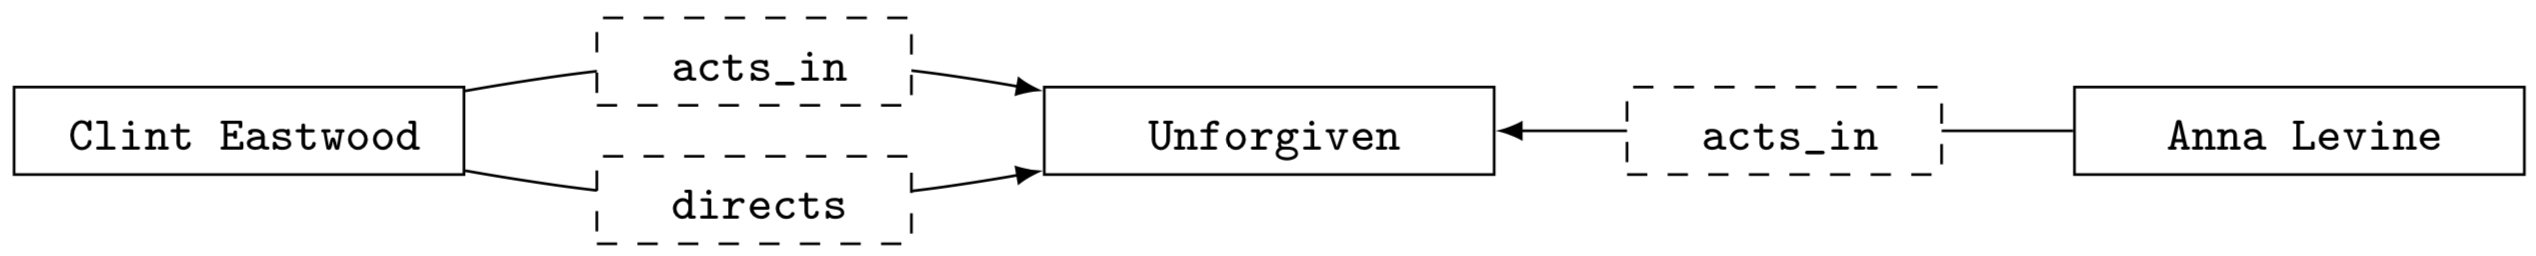
\includegraphics[width=\textwidth]{figures/edge_labelled_graph.png}
    \caption{An edge-labelled graph encoding basic movie information with dashed labels on edges\cite{2017ADatabases}}
    \label{fig:edge_labelled_graph}
\end{figure}

Since gMark generates directed edge-labelled graphs, we can amend definition \ref{def:edge_labelled_graph} by adding that a tuple $e \in E$ is ordered, and these edges may be called arrows or directed edges. For example, in a social network a directed edge $(A, knows, B)$ implies A knows B, but does not imply that B knows A.

Edge-labelled graphs do have limitations due to their simplicity. For example, it is not possible to label nodes. If you need to indicate what type a node is, you would need to create a new node with the name of the type and then create a directed "is" edge from the entity node to the type node. Various limitations of edge-labelled graphs can be worked around by simply creating more nodes and relationships to encode properties, but how does one encode that a person is born on a certain date? Creating nodes for every possible birthday and then creating "born on" relationships is certainly possible, but also very cumbersome and it greatly increases the size of the graph. It is also not possible to assign properties to the labelled edges, so if one wants to record properties of relationships such as the date the relationship is created, then that also requires more nodes and edges. Figure \ref{fig:edge_labelled_graph_downsides} shows a graph similar to the one in figure \ref{fig:edge_labelled_graph} but with extra nodes to encode various properties.

Another downside of edge-labelled graphs is that it is more difficult to indicate a schema. As per our example, a node for the person "Anna" may have an "is" relationship to the node "person" to indicate that Anna is a person. Anna may also have a "born on" relationship to the node "01-01-1988" to indicate she was born on that date. However, it is not clear in this way that being born on a certain date is in fact a property of being a person.

\begin{figure}
    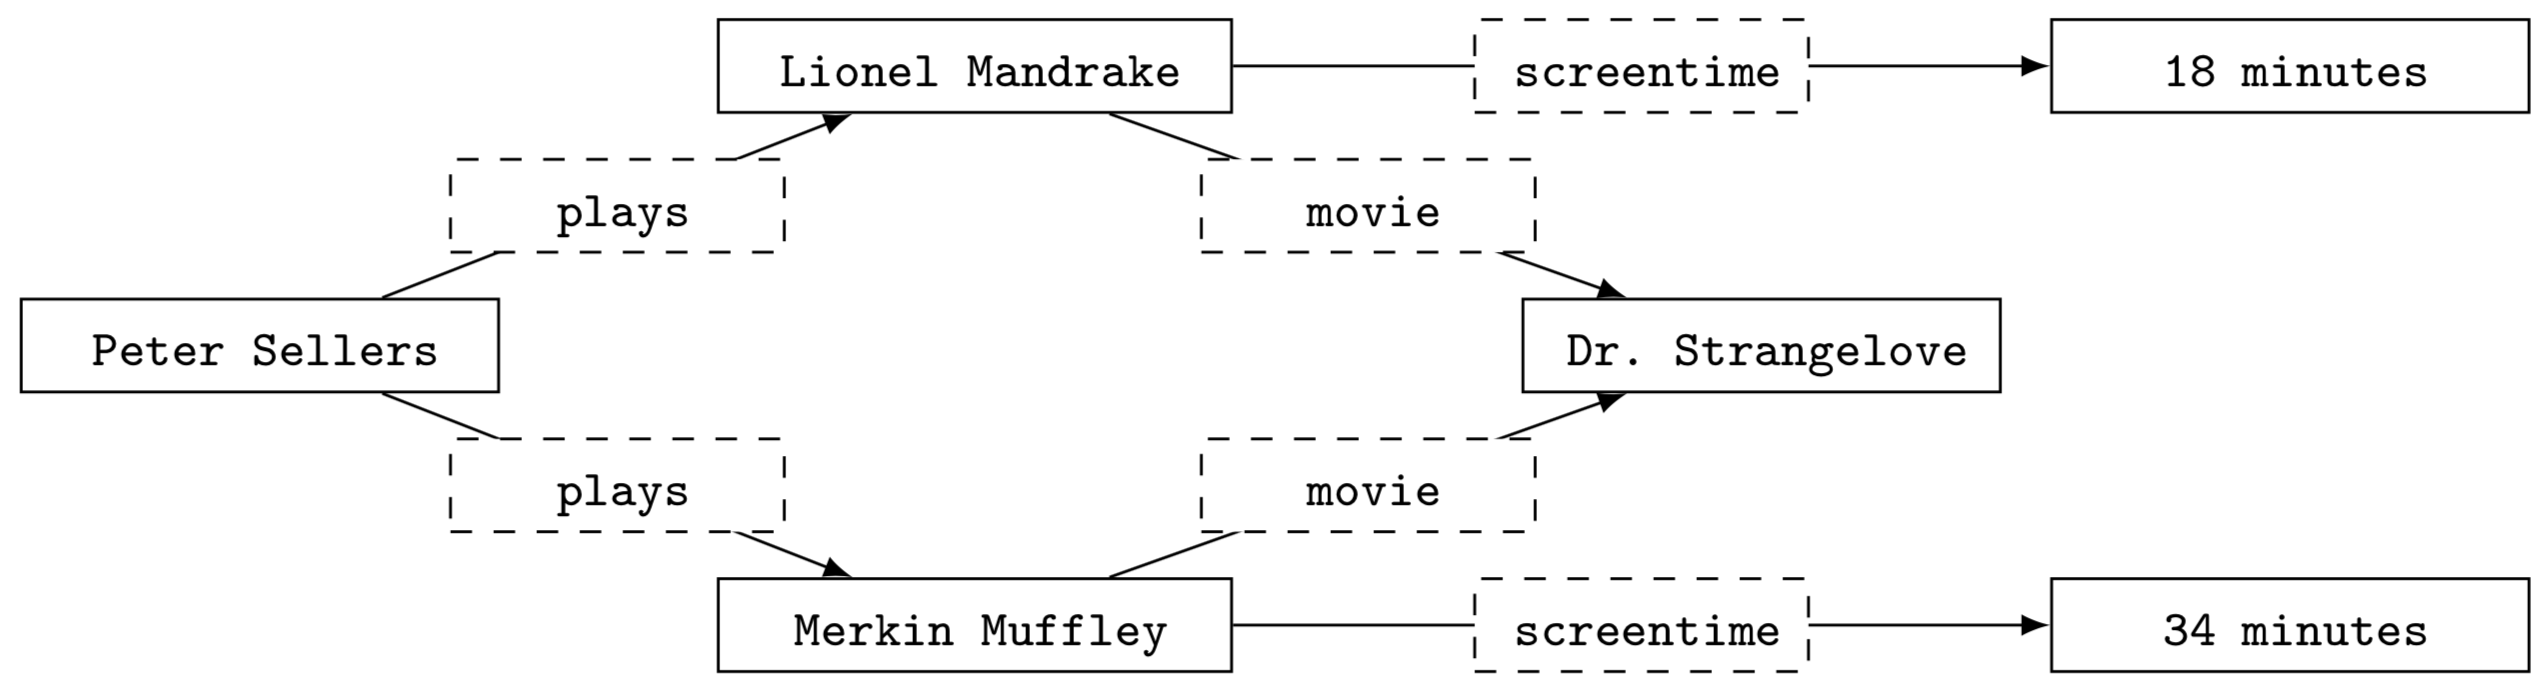
\includegraphics[width=\textwidth]{figures/edge_labelled_graph_downside.png}
    \caption{A version of figure \ref{fig:edge_labelled_graph} where extra nodes are used to encode properties \cite{2017ADatabases}}
    \label{fig:edge_labelled_graph_downsides}
\end{figure}